\chapter{Arbeitsumgebung}\label{ch:arbeitsumgebung}
In diesem Abschnitt wird der Arbeitsplatz und die Umbgebung, während der Probe-IPA, des Kandidaten beschrieben.
\section{Arbeitsplatz}\label{sec:arbeitsplatz}

\begin{figure}[H]
    \begin{center}
        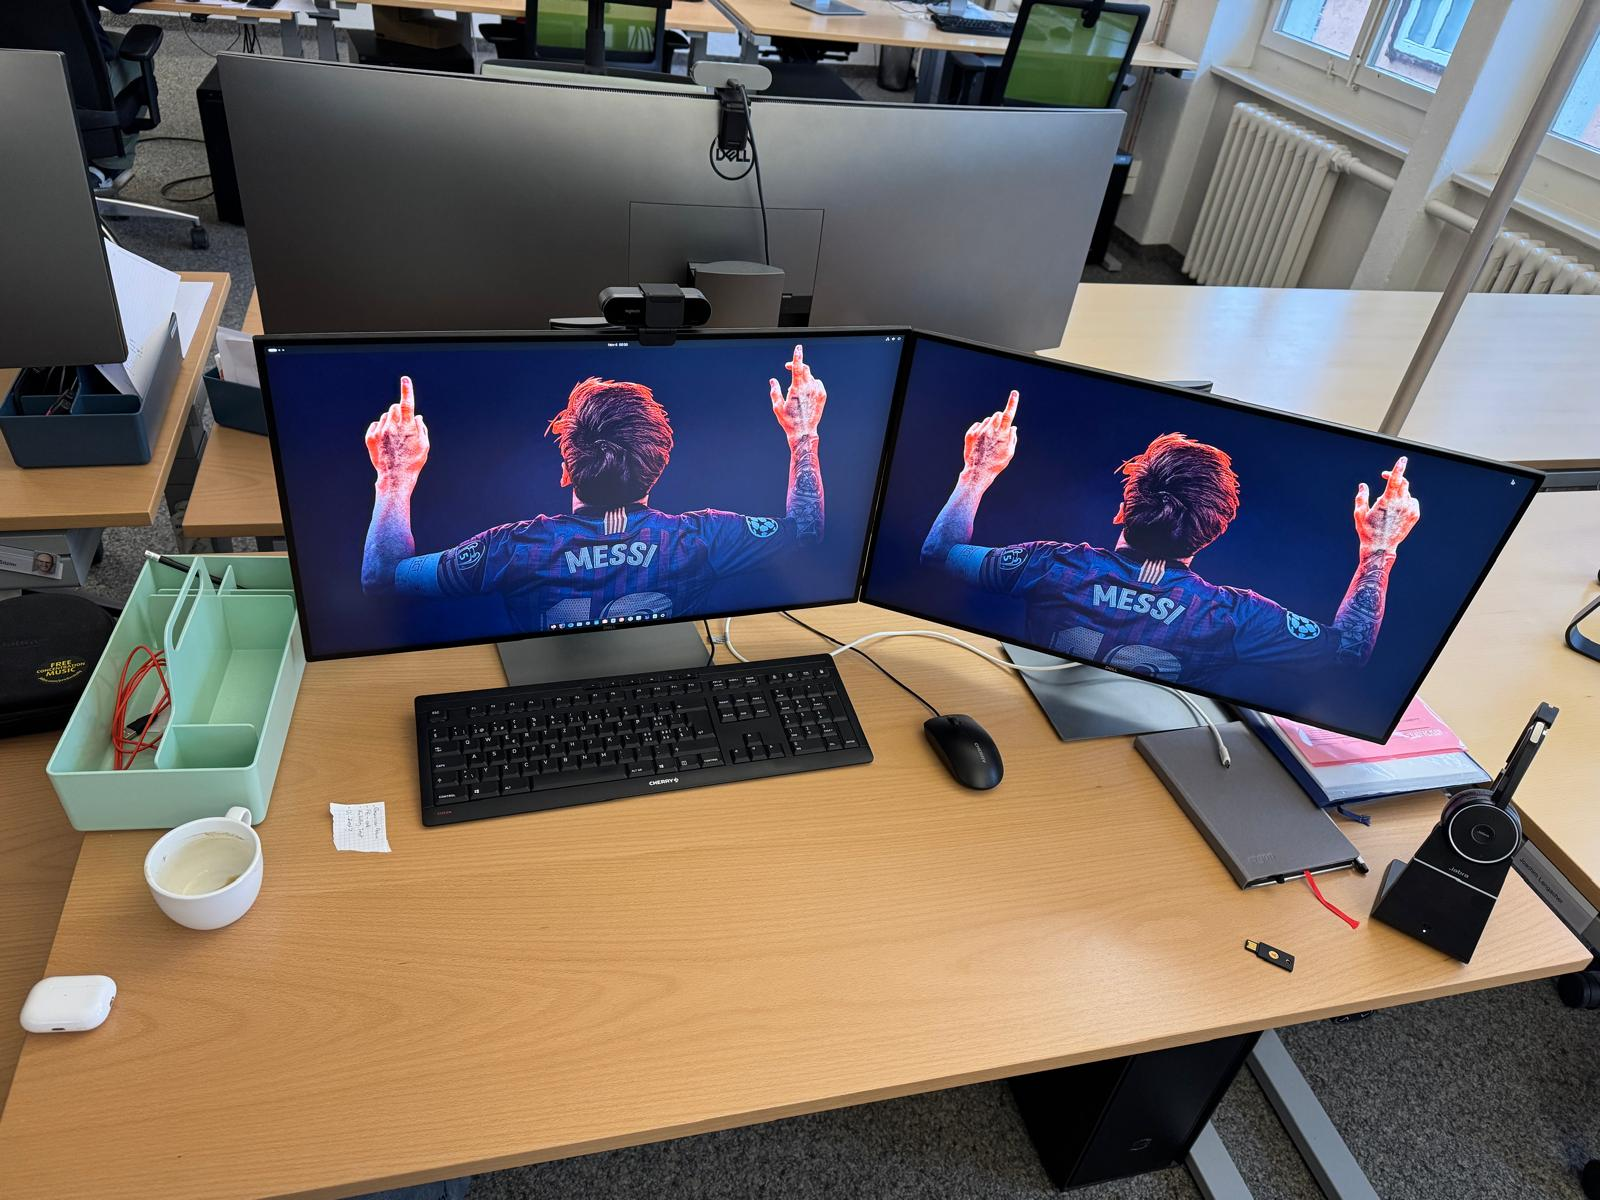
\includegraphics[width=0.8\textwidth]{ressourcen/arbeitsplatz}
        \caption[Arbeitsplatz]{Arbeitsplatz während der Probe-IPA}\label{fig:arbeitsplatz}
    \end{center}
\end{figure}

Da seit der Mitarbeit im IAM nie im Homeoffice gearbeitet wurde, findet auch die Probe-IPA wie gewohnt vor Ort statt. Der Desktop PC mit dem Betriebssystem Linux (Distribution Ubuntu) ist für die maximale Effizienz mit 2 Bildschirmen verbunden. Um im Grossraumbüro möglichst ungestört zu arbeiten, liegen dem Kandidaten ein Paar Airpods Pro mit Noise Cancelling vor.

\newpage \section{Verwendete Tools}\label{sec:verwendete-tools}
Die folgende Tabelle zeigt einen Überblick der wichtigsten Tools, welche für die Umsetzung der Probe-IPA verwendet wurden:

\renewcommand{\arraystretch}{1.5}
\begin{longtable}{|p{.22\textwidth}|p{.40\textwidth}|p{.38\textwidth}|}
    \hline
    \textbf{Tool} & \textbf{Einsatzzweck} & \textbf{Link} \\ \hline
    Intellij Ultimate           & Entwicklungsumgebung, zur Entwicklung des Features                   & \url{https://www.jetbrains.com/de-de/idea/}     \\ \hline
    TeXstudio           & Enticklungsumgebung für Latex, mit welchem die Dokumentation geschrieben wurde & \url{https://www.texstudio.org/}     \\ \hline
    Gerrit           & Quellcode Verwaltung & \url{https://www.gerritcodereview.com/}     \\ \hline
    Git          & Versionskontrollsystem & \url{https://git-scm.com/}     \\ \hline
    Jenkins & Automatisierte Testruns  & \url{https://www.jenkins.io/}     \\ \hline
    Outlook & Termin für den Expertenbesuch aufsetzen & \url{https://www.microsoft.com/de-ch/microsoft-365/outlook} \\ \hline
    
\end{longtable}
\renewcommand{\arraystretch}{1}
\newpage